%!TEX root = <main.tex>
\section{Introduction}
Deep convolutional neural networks (CNNs) \cite{alexnet, vggnet, resnet, inception} have revolutionized the computer vision field with even surpassing human level accuracies for some image recognition challenges such as ImageNet challenge~\cite{imagenet}.
Many of these successful pre-trained CNNs from computer vision challenges have been successfully re-purposed to be used in other real-world image recognition tasks, using a paradigm called \textit{transfer learning} \cite{transfer-learning-factors}.
In transfer learning, instead of training a CNN from scratch, one uses a pre-trained Deep CNN, e.g., ImageNet trained VGG, and fine tune it for the target problem using the target training dataset.
This approach avoids the need for a large training datasets, computational power and time which is otherwise a bottleneck for training a CNN from scratch.
As a result, this paradigm has enabled the wide adoption of deep CNN technology in variety of real world image recognition tasks in several domains including health care \cite{kermany2018identifying, islam2017abnormality}, agriculture \cite{mohanty2016using}, security \cite{arbabzadah2016identifying}, and sociology \cite{wang2017deep}.
Remarkably, United States Food and Drug Administration Agency has already approved the use of deep CNN based technologies for identifying diabetic retinopathy, an eye disease found in adults with diabetes.
It is also expected that above type of decision support systems will help the human radiologists in fulfilling their workloads efficiently and also provide a remedy to the shortage of qualified radiologists globally \cite{radiologistshortage}.

However, despite their many success stories, one of the major criticisms for deep CNNs and deep neural networks in general is the black-box nature of how they make predictions.
In order to apply deep CNN based techniques in critical applications such as health care, the decisions should be explainable so that the practitioners can use their human judgment to decide whether to rely on those predictions or not \cite{jung2017deep}.

\begin{figure}[t]
  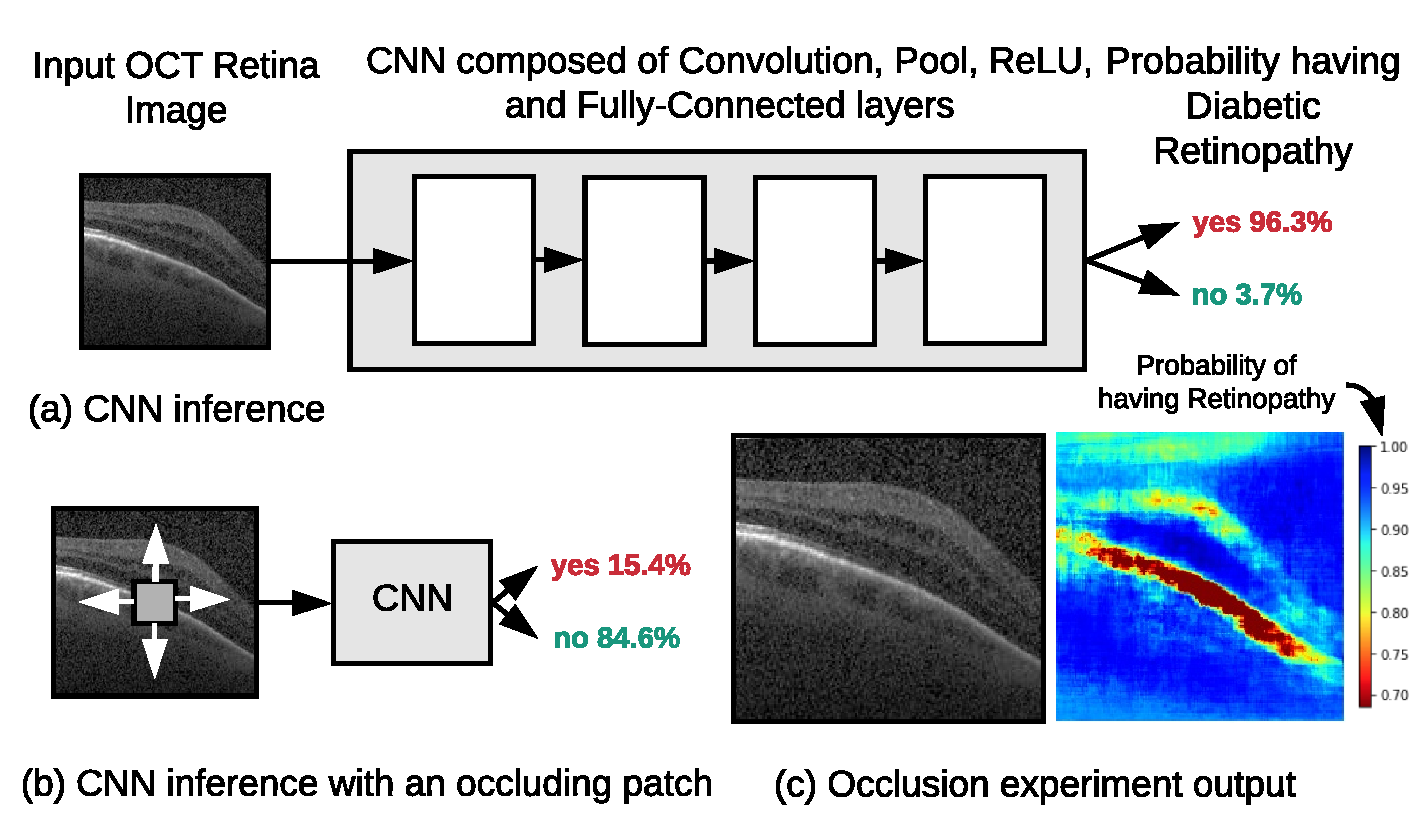
\includegraphics[width=\columnwidth]{./images/krypton_overview}
  \caption{(A) Simplified representation depicting how OCT images are used for predicting Diabetic Retinopathy using CNNs. (B) Occluding parts of the OCT image changes the predicted probability for the disease. (C) By systematically moving patch along vertical and horizontal axes an output heat map is generated where each individual value corresponds to the predicted disease probability when the occlusion patch was placed on that position.}
  \label{fig:krypton_overview}
\end{figure}

In order to improve the explainability of deep CNN predictions several approaches have been proposed.
One of the most widely used approach in image recognition tasks is occlusion experiments \cite{zeiler2014visualizing}.
In occlusion experiments, as shown in Figure~\ref{fig:krypton_overview} (B), a square patch usually of gray or black color is used to occlude parts of the image and record the change in the predicted label probability.
By systematically striding this patch horizontally and vertically one or two pixels at a time over the image a sensitivity heat map for the predicted label similar to one in Figure~\ref{fig:krypton_overview} (C) can be generated.
Using this heat map, the regions in the image which are highly sensitive (or highly contributing) to the predicted class can be identified (corresponds to red color regions in the sensitivity heat map shown in Figure~\ref{fig:krypton_overview} (C)).
This localization of highly sensitive regions then enables the practitioners to get an idea of the the prediction process of the deep CNN.

\textbf{\textit{Example:}} Consider a radiologist who is examining Optical Coherence Tomography (OCT) images of the retina to identify potential diabetic retinopathy patients.
The radiologist is recently given access to a deep CNN based clinical decision support system (CDSS) to identify potential images with diabetic retinopathy. 
It predicts the probability whether a retina image depicts a diabetic retinopathy case.
She uses the CDSS for two main purposes: 1) as a cross checker while manually inspecting the retinal images, and 2) to prioritize potentially sever cases from a backlog of retina images.
In both situations in addition to predicting the existence of the disease, the radiologist would like to have an explanation for the basis on which the CDSS makes the prediction, using the occlusion based explainability approach, to decide whether the pathological regions identified by the CDSS are correct and to ultimately whether to rely on the CDSS decision. Similar examples arise in number of other heal care applications such as chest X-ray examination for identifying pneumonia cases and X-ray based child bone age assessment.

However, occlusion experiments are highly compute intensive and time consuming as each patch super imposition is treated as a new image and requires a separate CNN inference.
In this work our goal is to apply database inspired optimizations to the occlusion based explainability workload to reduce both the computational cost and runtime taken for an experiment.
This will also make occlusion experiments more amenable for interactive diagnosis of CNN predictions.
Our main motivation is based on the observation that when performing CNN inference corresponding to each individual patch position, there are lot of redundant computations which can be avoided.
To avoid redundant computations we introduce the notion of \textit{incremental inference} of deep CNNs which is inspired by the incremental view maintenance approach which is heavily studied in the context of relational databases.

Due to the overlapping nature of how a convolution kernel would operate (details to follow in Section \ref{sec:preliminaries}), the size of the modified patch will start growing as it progress through more layers in a CNN and reduce the amount of redundant computations.
However at deeper layers the effect over patch coordinates which are radially further away from the center of the patch position will be diminishing.
Our second optimization is based on this observation where we apply a form of \textit{approximate inference} which applies a \textit{propagation threshold} to limit the growth of the updating patch.
We show that by applying propagation thresholds, a significant amount of computation redundancy can be retained.

The third optimization is also a form of \textit{approximate inference} which we refer as \textit{adaptive drill-down}.
In most occlusion experiment use cases, such as in medical imaging, the object or pathological region of interest is contained in a relatively small region of the image.
In such situations it is unnecessary to inspect the original image at the same high resolution of striding the occluding patch one or two pixels at a time, at all image locations.
In adaptive drill-down approach, first a low resolution heatmap is generated with a larger occluding patch and a larger stride with relatively low computational cost and only the interested regions will be inspected further with a smaller occluding patch and a smaller stride to produce a higher resolution output.
This two stage process also reduces the runtime of occlusion experiments.

Unlike the \textit{incremental inference} approach which is exact, \textit{propagation thresholding} and \textit{adaptive drill-down} are approximate approaches. They essentially trade-off accuracy of the generated sensitivity heat map compared to the original, in favor of faster runtime.
These changes in accuracy in the generated heat map will be visible all the way from quality differences which are almost indistinguishable to the human eye to drastic structural differences, depending on the level of approximation.
This opens up an interesting trade-off space of quality/accuracy versus runtime. \system~ expects the user to define the required level of quality for the generated heat maps by specifying the Structural Similarity Index (SSIM) (explained in Section \ref{sec:preliminaries}) quality metric.
The system will then automatically tune it's \textit{approximate inference} configuration values to yield the expected quality level during an initial tuning phase.

Finally, we have implemented \system~ on top of PyTorch deep learning toolkit by extending it by adding custom implementations of incremental and approximate inference operators.
It currently supports VGG16, ResNet18, and InceptionV3 both on CPU and GPU environments, which are three widely used deep CNN architectures for transfer learning applications.
We evaluate our system on three real-world datasets, 1) diabetic retinopathy (DR), 2) chest X-ray (CX), and 3) hand \& wrist X-Ray (HX), and show that \system~ can result in up to 10x speedups with hardly distinguishable quality differences in the generated occlusion heat maps. While we have implemented \system~ on top of PyTorch toolkit, our work is largely orthogonal to choice of the deep learning toolkit; one could replace PyTorch with TensorFlow, Caffe2, CNTK, MXNet, or implement from scratch using C/CUDA and still benefit from our optimizations.
Overall, this paper makes the following contributions:

\begin{itemize}
	\item To the best of our knowledge, this is the first paper to study
\end{itemize}

\vspace{2mm}
\noindent \textbf{Outline.} The rest of this paper is organized as follows.
